\chapter{Alimentation Flyback}

La maquette d’étude comprend, outre le circuit de commande du transistor, le montage suivant :

\begin{figure}[h]
\centering
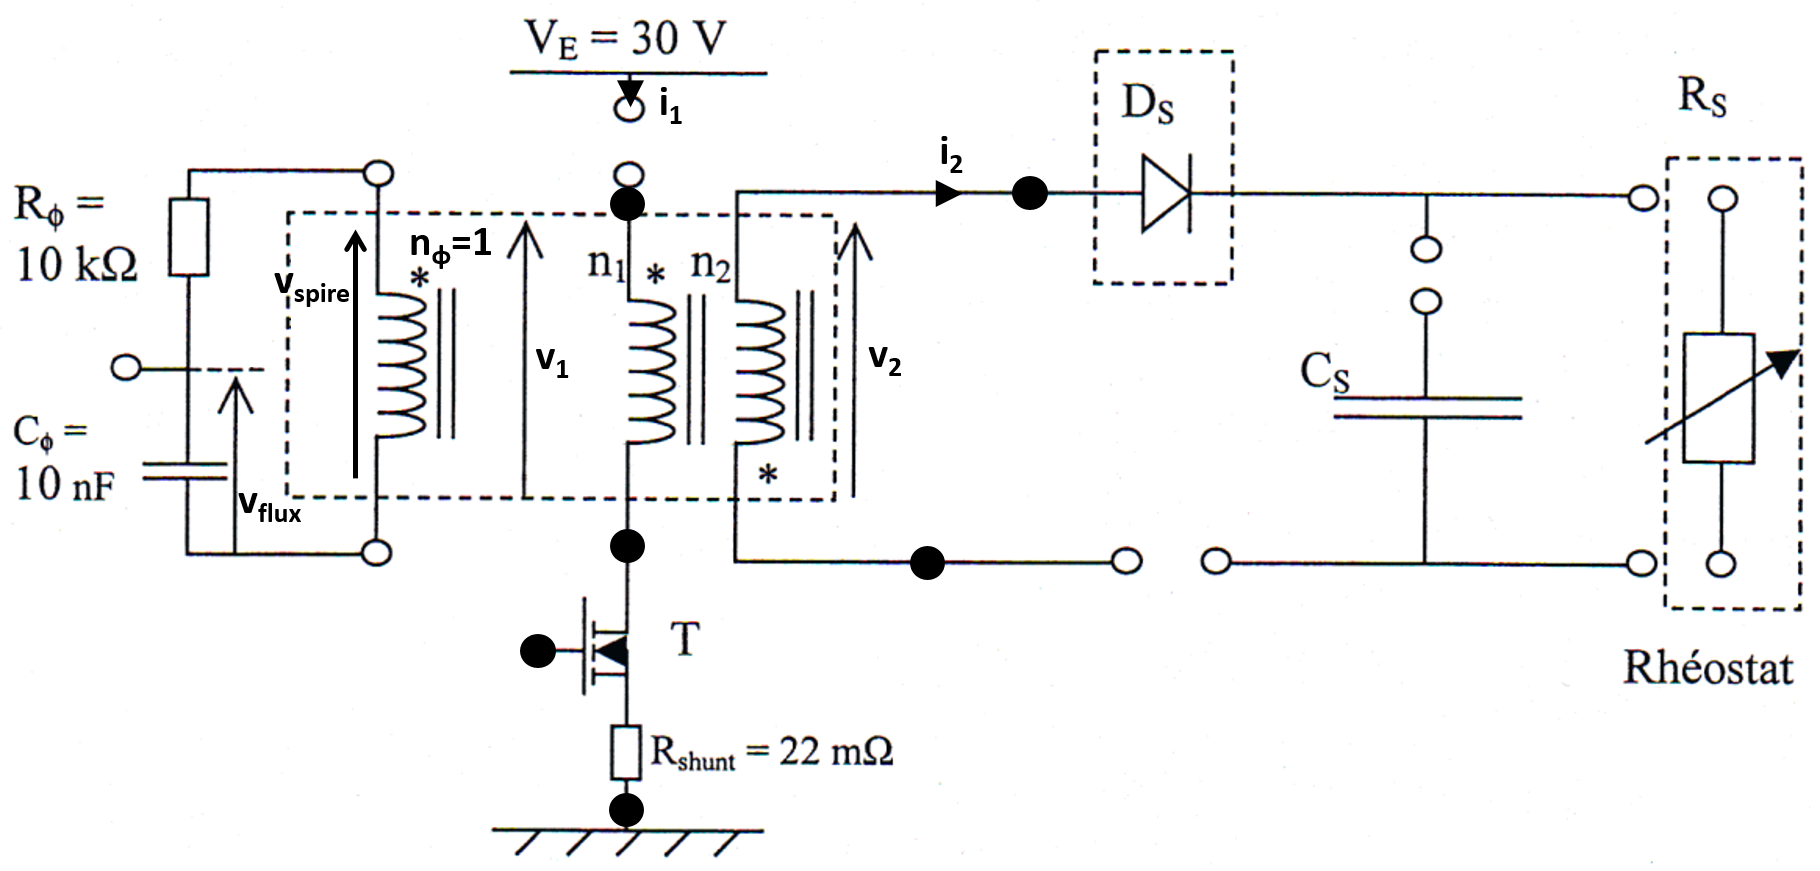
\includegraphics[width=\linewidth]{TP_Flyback/fig/Schema_Flyback.png}
%\caption{Simplified internal control}
\end{figure}

Des pointes de tests $\bullet$ permettent de visualiser les différents signaux, notamment le signal de commande du transistor MOSFET.

Les 3 enroulements sont sur le même noyau magnétique ETD29/16/10 réalisé avec une ferrite de type N27 dont la document est en annexe. Ce noyau peut être muni d’un entrefer réglé par des cales amagnétiques. Dans ce cas, la relation entre l’épaisseur $s$ de l’entrefer et la valeur $A_L$ de l’inductance spécifique est donnée par la relation suivante où $K_1$ et $K_2$ sont deux constantes données dans la documentation :
$$s=(\dfrac{A_L}{K_1})^{\dfrac{1}{K_2}}$$

Les liaisons manquantes devront être réalisées par des ``cavaliers'' permettant de visualiser les courants par l’utilisation de sondes appropriées. Le rhéostat de charge peut être de 250 $\Omega$ ou 330 $\Omega$ indifféremment et on veillera à \underline{\textbf{ne pas brancher la tension $V_E$ sans la présence}} \underline{\textbf{de cette charge}}.

On notera la présence d’un circuit de mesure du flux réalisé par une spire unique reliée à un circuit R-C intégrateur. La tension $v_{flux}$ permet donc de visualiser l’ondulation du flux dans le circuit magnétique.

\newpage
Le dispositif de commande du transistor est représenté sur la figure ci dessous :

\begin{figure}[h]
\centering
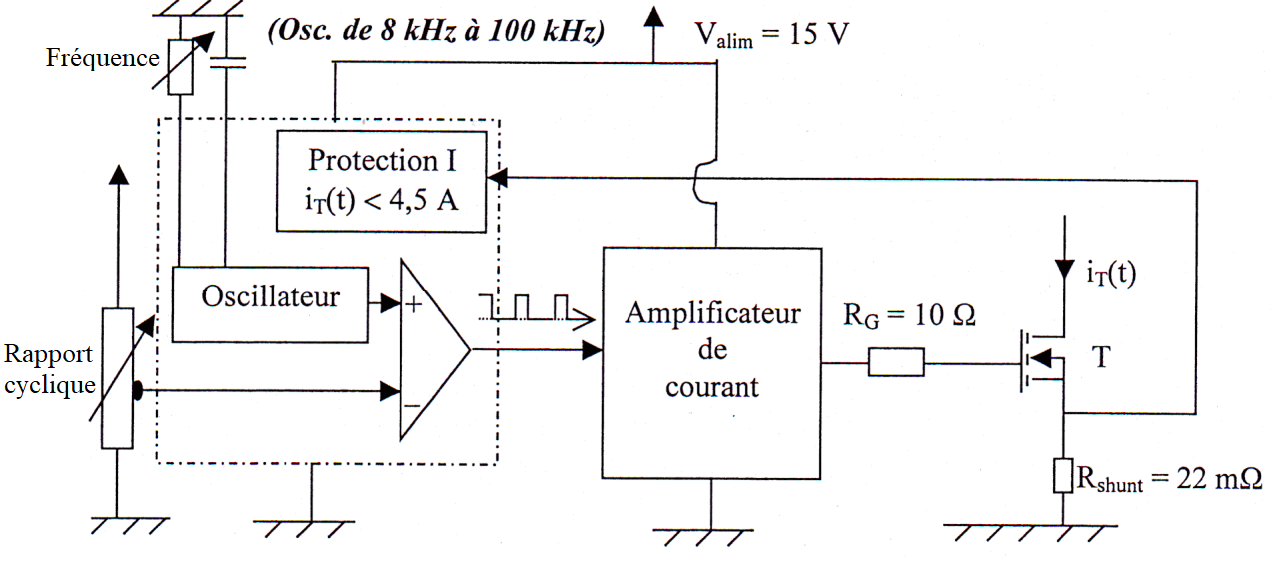
\includegraphics[width=\linewidth]{TP_Flyback/fig/Control_Flyback.png}
%\caption{Simplified internal control}
\end{figure}

Un potentiomètre permet de régler la fréquence (ne pas descendre en dessous de 15 kHz), un second permet de régler le rapport cyclique. Ce dernier est muni d’une limitation de courant active réglée à 4,5A et réalisée par la mesure de tension sur un shunt de 22 m$\Omega$. L’alimentation de cette commande est réalisée par une source de tension indépendante de valeur $V_{alim} = 15 V$.

\newpage
\section{Préparation}

On suppose que le transistor est commandé par un signal PWM de rapport cyclique $\alpha=0.25$. On suppose également que le convertisseur fonctionne en \textbf{régime de démagnétisation totale} pour le transformateur. La tension d'entrée $V_E$ est supposée constante. On étudiera pour la préparation uniquement le \underline{régime permanent}.

\begin{enumerate}
\item Compléter les chronogrammes ci-dessous en traçant : 
\begin{itemize}
\item le flux $\varphi$ dans le transformateur
\item le courant $i_1$ délivré par l'alimentation
\item le courant $i_2$ dans la diode
\item la tension $v_2$ en sortie du transformateur
\end{itemize}


\begin{figure}[h]
\centering

\includegraphics[width=0.7\linewidth]{TP_Flyback/fig/prepa.png}
%\caption{Simplified internal control}
\end{figure}

\item On suppose que la constante de temps du filtre $R_\phi-C_\phi$ est grande devant la période de découpage du hacheur. Montrer que $v_{flux}$ permet de visualiser l'ondulation de flux dans la transformateur. Déterminer l'ondulation de flux $\Delta \varphi$ en fonction de $\alpha$, $T$ et la valeur de $v_{spire}$ sur l'intervalle $0<t<\alpha T$.
\end{enumerate}


%%%%%%%%%%%%%%%%%

\newpage
Durant tout le TP, les précautions suivantes devront être prises :

\begin{itemize}
\item utiliser deux sources indépendantes pour réaliser $V_{alim}$ et l’alimentation ``de puissance'' $V_E$ : \textbf{on
règlera soigneusement la limitation de courant de celle-ci à 2 A}
\item laisser la tension $V_{alim}$ présente durant toute la séance mais baisser la tension $V_E$ à chaque
modification de branchement
\item ne pas abaisser la fréquence de découpage en dessous de 15 kHz
\item lorsque plusieurs mesures de tensions sont réalisées en même temps avec une sonde de tension, \textbf{attention à ne pas réaliser de court-circuit}. En effet, les sondes de tensions ne sont pas isolées entre elles, les références de potentiel des sondes sont donc liées via l'oscilloscope
\end{itemize}

\section{Étude magnétique, formes d’onde}

On effectuera les mesures suivantes avec le rhéostat de charge à sa valeur maximale (charge réduite) et en veillant à travailler en régime de démagnétisation totale, pour un rapport cyclique voisin de sa valeur maximale.

\begin{enumerate}
\item Régler la fréquence de découpage à 50 kHz et le rapport cyclique à sa valeur maximale (que l’on notera). Observer la tension aux bornes de la spire de mesure du flux $v_{spire}$ ainsi que la tension $v_{flux}$. En déduire l’excursion crête à crête $\Delta B$ de l'induction magnétique dans le circuit en s’aidant de la documentation ($\Delta B = B_{max} – B_{min}$).
\item Par comparaison des tensions $v_{spire}$ et $v_1$, puis $v_2$, déterminer les nombres de spires $n_1$ et $n_2$.
\item Observer simultanément les courants $i_1$ et $i_2$ et les comparer à l’évolution du flux.
\item En déduire la valeur de l’inductance magnétisante au primaire, notée $L_1$.
\item A partir des mesures de $n_1$ et $L_1$ et en utilisant la documentation, déterminer la valeur de l’inductance spécifique $A_L$ puis l’épaisseur de l’entrefer. Quel est le rôle de cet entrefer ?
\end{enumerate}

\newpage
\section{Courbes statiques}

Le but de ces mesures est de relever le réseau des caractéristiques statiques en sortie de l’alimentation. La fréquence de découpage est dans un premier temps maintenue constante égale à 50 kHz.

\begin{enumerate}
\item Pour plusieurs valeurs du rapport cyclique (par exemple $\alpha_{max}$, 0.3, 0.2 et 0.1), modifier la résistance du rhéostat de charge pour faire varier le courant moyen débité entre sa valeur minimale (obtenue avec le rhéostat au maximum) et une valeur maximale de 2 A. Relever alors les valeurs moyennes du courant débité par l’alimentation de puissance $V_E$, $I_E$, du courant de sortie, $I_S$, et de la tension de sortie, $V_S$. Noter soigneusement le point de fonctionnement correspondant au changement de régime de l’alimentation vis à vis de la démagnétisation.
\item En déduire le tracé des caractéristiques $V_S(I_S)$ et $P_S(I_S)$ (puissance de sortie) paramétrées par $\alpha$. Tracer également les caractéristiques de transfert en puissance $P_S(P_E)$ et en déduire le rendement. Faire apparaître les zones de fonctionnement en démagnétisation partielle et en démagnétisation totale.
%\item Afin de maintenir l’alimentation en régime critique, il est possible de modifier la fréquence de découpage. Ceci est en général réalisé au moyen d’une commande auto-oscillante mais on peut simuler ce fonctionnement de la façon suivante : on réglera la fréquence de découpage pour maintenir la valeur moyenne de la tension de sortie constante alors que le rapport cyclique reste constant, réglé à $\alpha_{max}$, ceci pour différentes valeurs du rhéostat de charge. Pour réaliser facilement ces mesures, on procédera ``à l’envers'' en réglant d’abord une valeur de fréquence de découpage puis en modifiant la valeur du rhéostat pour obtenir la tension de sortie souhaitée, par exemple $V_S = 40 V$. Relever alors le point de fonctionnement, i.e. la valeur moyenne du courant de sortie $I_S$ et la fréquence de découpage.

%\item Observer les formes d'onde de la tension $V_{CE}$ aux bornes du transistor et du courant $i_1$ le traversant. En déduire les contraintes sur la transistor.
\end{enumerate}

\section{Mesures complémentaires}

Laisser le rhéostat de charge à sa valeur maximale et la fréquence de découpage à 50 kHz.

\begin{enumerate}
\item Observer simultanément le courant $i_1$ et la tension aux bornes du transistor $v_T$. En déduire les contraintes subies par ce transistor.% et évaluer ses pertes en commutation et en conduction.
\item Observer simultanément le courant dans le condensateur de filtrage $I_{CS}$ et la tension de sortie $v_S$. En déduire la valeur du condensateur de filtrage $C_S$.
\end{enumerate}
